\documentclass[letterpaper,12pt]{article}
\usepackage{enumitem}
\usepackage[margin=1.0in]{geometry}
\usepackage{setspace}
\newcommand\textbox[1]{%
  \parbox{.333\textwidth}{#1}%
}
\usepackage{paralist}
\renewenvironment{itemize}[1]{\begin{compactitem}#1}{\end{compactitem}}
\renewenvironment{enumerate}[1]{\begin{compactenum}#1}{\end{compactenum}}

\usepackage{graphicx}
\usepackage{amsmath}

\usepackage{listings}

\setcounter{secnumdepth}{0}


\setlength\parindent{0pt}
\setlength{\parskip}{6pt plus 1pt minus 1pt}


\def\changemargin#1#2{\list{}{\rightmargin#2\leftmargin#1}\item[]}
\let\endchangemargin=\endlist 

\usepackage{titlesec}

\usepackage{float}
\usepackage{setspace}

\usepackage{tocloft}

\setlength\cftparskip{4pt}

\newcommand\blfootnote[1]{%
  \begingroup
  \renewcommand\thefootnote{}\footnote{#1}%
  \addtocounter{footnote}{-1}%
  \endgroup
}



\usepackage{color}

\definecolor{dkgreen}{rgb}{0,0.6,0}
\definecolor{gray}{rgb}{0.5,0.5,0.5}
\definecolor{mauve}{rgb}{0.58,0,0.82}

\lstset{frame=tb,
  language=Java,
  aboveskip=3mm,
  belowskip=3mm,
  showstringspaces=false,
  columns=flexible,
  basicstyle={\footnotesize\ttfamily},
  numbers=none,
  numberstyle=\tiny\color{gray},
  keywordstyle=\color{blue},
  commentstyle=\color{dkgreen},
  stringstyle=\color{mauve},
  breaklines=true,
  breakatwhitespace=true,
  tabsize=3
}

\newcommand{\tabitem}{~~\llap{\textbullet}~~}

\usepackage{multirow}
\usepackage{pbox}

\usepackage[bottom]{footmisc}
\usepackage{url}

\urlstyle{same}

\usepackage{menukeys}

\usepackage{lmodern}

\usepackage{tikz}
\usetikzlibrary{calc}

\usepackage{fancyhdr}
\fancyhead[L]{GroceryHelper}
\fancyhead[R]{Software User Manual}




\begin{document}

\thispagestyle{empty}

\begin{titlepage}



\vspace*{\fill}

\begin{center}


\includegraphics[scale=0.7]{LOGO.png}


\begin{LARGE}

\textbf{GroceryHelper\Large{\textsuperscript{TM}}}

\textbf{Software User Manual}


\vspace{0.1in}



\end{LARGE}


\vspace{0.5in}



\begin{Large}
\textit{The Wacky Wozniaks Company}
\end{Large}

\begin{large}
\textit{Hyun Choi, Luke Giacalone, and Julia McClellan}
\end{large}



\end{center}



\vspace*{\fill}

\end{titlepage}




\pagebreak

\thispagestyle{plain}
\setcounter{page}{2}

\tableofcontents

\pagebreak

%\newgeometry{top=0.75in,bottom=0.75in,left=0.75in,right=0.75in}






\pagebreak

\newgeometry{margin=0.8in, top=1.0in}

\pagestyle{fancy}


\section{Introduction}

GroceryHelper{\footnotesize\textsuperscript{TM}} is a highly versatile, cross-platform tool that keeps track of inventories of consumable products and generates a shopping list if and when such consumable objects are running low. Items can be sorted by location or by kind in different inventories. By setting the lower and upper limit of acceptable quantities of each item, GroceryHelper is able to create and export to a file, an email, or a printer a conveniently formatted list of items that the user must purchase. Thus, this application offers a 21$^\text{st}$ century upgrade to the age-old concept of the ``grocery list'' and makes shopping for household items more convenient for everyone.



\section{System Requirements}
As a Java application, GroceryHelper is compatible with the vast majority of computers, including relatively outdated operating systems (e.g. Windows Vista) as well as less common ones (e.g. Linux$^\text{\textregistered}$). The program was built to be fully functional with versions of Java Runtime Environment (JRE) as old as JRE 6. Older Java versions may still be able to run GroceryHelper, but this functionality has not been tested by the Wacky Wozniaks Company.



The Oracle corporation has outlined the following system requirements for the installation of Java 7:\footnote{\url{https://www.java.com/en/download/help/sysreq.xml}}

\begin{table}[H]
\centering
\label{my-label}
\begin{tabular}{|c|c|p{10cm}|}
\hline
\multicolumn{2}{|c|}{Component}             & \multicolumn{1}{c|}{Minimum Required}                                                                                                                                                                                                                                                                                                                                                                                                                                                         \\ \hline
\multirow{3}{*}[-0.5em]{\pbox{2cm}{\centerline{Operating}\centerline{System}}} & Windows & \begin{tabular}[c]{@{}l@{}}\tabitem Windows 10 (7u85 or higher)\\ \tabitem Windows 8.x (Desktop)\\ \tabitem Windows 7 SP1\\ \tabitem Windows Vista SP2\\  \tabitem Windows Server 2008 SP2 and 2008 R2 SP1 (64-bit)\\ \tabitem Windows Server 2012 (64-bit) and 2012 R2 (64-bit)\\ \tabitem Windows XP*\end{tabular}                                                                                                                                   \\ \cline{2-3} 
                                  & Mac     & \tabitem Intel-based Mac running OS X 10.7.3 (Lion) or later                                                                                                                                                                                                                                                                                                                                                                                                                                  \\ \cline{2-3} 
                                  & Linux & \begin{tabular}[c]{@{}l@{}}\tabitem Various, please refer to footnoted link \end{tabular} \\ \hline
\multicolumn{2}{|c|}{CPU}                   & Pentium 2 266 MHz processor                                                                                                                                                                                                                                                                                                                                                                                                                                                                   \\ \hline
\multicolumn{2}{|c|}{Memory (RAM)}          & 128 MB                                                                                                                                                                                                                                                                                                                                                                                                                                                                                        \\ \hline
\multicolumn{2}{|c|}{Disk Space}            & 126 MB                                                                                                                                                                                                                                                                                                                                                                                                                                                                                        \\ \hline
\multicolumn{2}{|c|}{Miscellaneous}         & \begin{tabular}[c]{@{}p{10cm}@{}}\tabitem To open exported Microsoft Word (.docx) documents, Microsoft Word 2007 or a later version must be installed\\ \tabitem To print the shopping list, a printer must be properly configured and installed to the computer.
\end{tabular}                                                                                                                                                                                                                    \\ \hline
\end{tabular}
\end{table}

*Note: As of April 8, 2014, Microsoft Corporation has halted support of Windows XP, and thus Oracle has removed it as an officially supported platform. While users may still be \textit{able} to run Java programs on Windows XP, they do so at their own risk and without support from Oracle or the Wacky Wozniaks Company.


\section{Getting Started}

GroceryHelper is offered in three versions, all with identical functionality. A \verb|.exe| executable file is provided for users who use a computer with Windows. A \verb|.app| application is provided for users who use a Macintosh computer. Finally, a \verb|.jar| Java executable file is also provided for users that run a different operating system, such as Linux, Unix, or variants thereof.


\section{Using GroceryHelper}

When GroceryHelper is run for the first time, a window resembling the following screenshot will pop up, along with a message.\\

\centerline{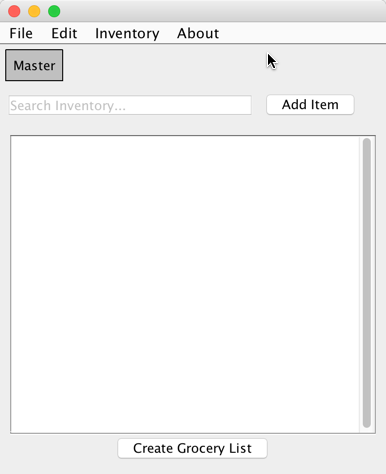
\includegraphics[scale=0.5]{08.png}}

\vspace{0.1in}

\centerline{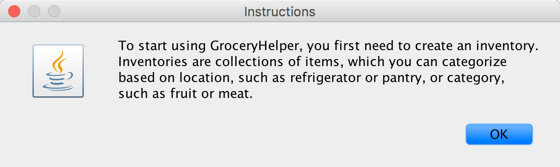
\includegraphics[scale=0.5]{05.png}}


\subsection{Your Inventories}

GroceryHelper maintains lists of products within different inventories. Each inventory could represent a location, such as a refrigerator or a pantry, or a type of item, such as fruit or meat. Each inventory can be viewed separately, and all items can be viewed in the Master inventory. Tabs at the top of the window provide a convenient and intuitive way to navigate between inventories.


	\subsubsection{Adding Inventories}

There are three simple ways to create and add an inventory:

\begin{enumerate}
\item Navigate to \menu[,]{File, New, Inventory...}.


\item Navigate to \menu[,]{Inventory, New...}.


\item Use the keyboard shortcut \keys{\ctrlwin + I} on Windows or \keys{\cmd + I} on Mac. \\

\end{enumerate}



\centerline{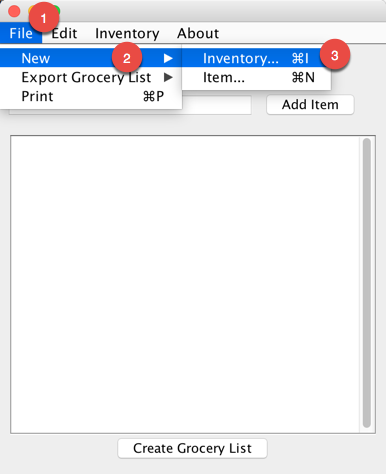
\includegraphics[scale=0.5]{06.png}}

Regardless of the method used, a window will pop up prompting for a name for the new inventory. The name must not be identical to that of any of the existing inventories, including the Master inventory. Once a unique name has been chosen, a tab for the new inventory will be added to the window.\\

\centerline{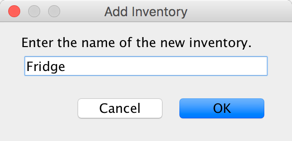
\includegraphics[scale=0.65]{02.png}}

	\subsubsection{Removing Inventories}
	
	
	There are two ways to remove an inventory:

\begin{enumerate}
\item Navigate to \menu[,]{Inventory, Remove}.


\item Use the keyboard shortcut \keys{\ctrlwin + R} on Windows or \keys{\cmd + R} on Mac. \\

\end{enumerate}	
	
\centerline{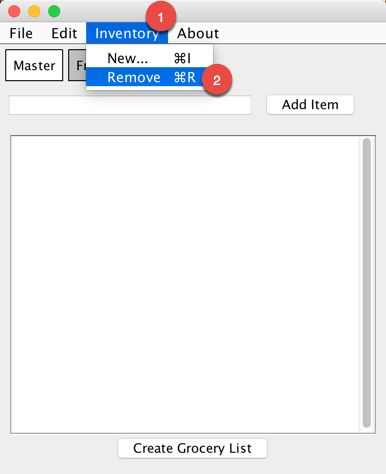
\includegraphics[scale=0.5]{12.png}}


Regardless of the method used, the currently displayed inventory will be removed. However, the Master inventory cannot be removed. If this operation is attempted, a notification will be displayed and no action will be taken.

		

	\subsubsection{Searching Inventories}
To search for an item within an inventory, use the search bar right above the list of items. The search feature can also be accessed with the keyboard shortcut \keys{\ctrlwin + F} on Windows or \keys{\cmd + F} on Mac.\\

\centerline{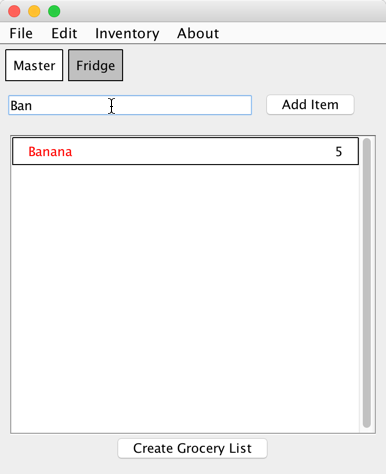
\includegraphics[scale=0.5]{18.png}}

As each character is entered into the search bar, all items with names that contain the text currently entered in the search bar will be displayed. The search bar only searches within the currently displayed inventory. To search through all inventories, simply search for an item in the Master inventory.

	\subsection{Your Items}
Each item contained in the inventory represents a specific product. Each item must have a unique name (i.e. no two items across all inventories can have the same name). A record is kept of the quantity of each item, which will be updated by the user each time an item is consumed or acquired. An item has two additional attributes: a minimum limit and a maximum limit.



If the quantity of the item falls lower than the minimum limit of the item, GroceryHelper will automatically add the item to the grocery list. The grocery list will display the quantity of that item the user must purchase to replenish the stock to the maximum limit.

	\subsubsection{Adding Items}
Similar to inventories, there are three ways to add items. Items will be added to the currently selected inventory.

\begin{enumerate}
\item In the menu bar, navigate to \menu[,]{File, New, Item...}.
\item An item can also be added with the \menu{Add Item} button directly adjacent to the search bar. 
\item Finally, an item can be added with the keyboard shortcut \keys{\ctrlwin + N} on Windows or \keys{\cmd + N} on Mac.


\end{enumerate}


Note: An item must be entered to a specific inventory; an item \textit{cannot} be directly entered into the Master inventory. If the Master inventory is currently selected, a window will first pop up asking for the selection of another inventory to which the item should be added.\\



\centerline{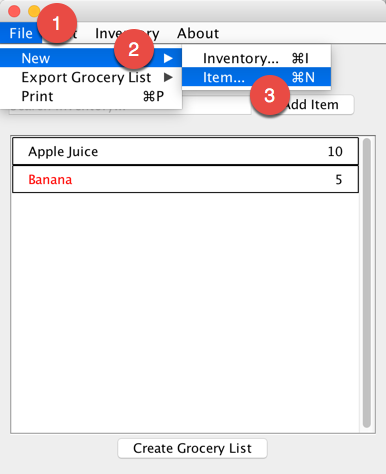
\includegraphics[scale=0.5]{10.png}}


Regardless of the method used, a new window will pop up to allow the user to add an item.\\

\centerline{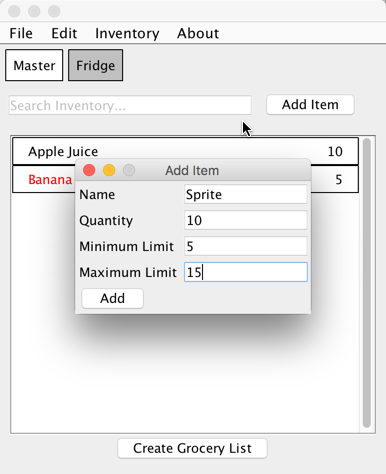
\includegraphics[scale=0.5]{04.png}}

There are four fields in the frame to add information about the item. All fields are required. The name of the item cannot be the same as any other item currently in any inventory. If text was entered in the search bar prior to adding an item, it will automatically be filled in as the name for the new item. The quantity must be an integer greater than or equal to zero. The minimum limit must also be an integer greater than or equal to one. Finally, the maximum limit must be an integer greater than one. Once all of these fields are complete, click the \menu{Add} button to add the item to the selected inventory. If any field is completed incorrectly, an message will be displayed with instructions on how to fix the values.


		\subsubsection{Modifying Items}
To modify an item's attributes, click on its name in the display. A window will pop up with information about that item. 

\centerline{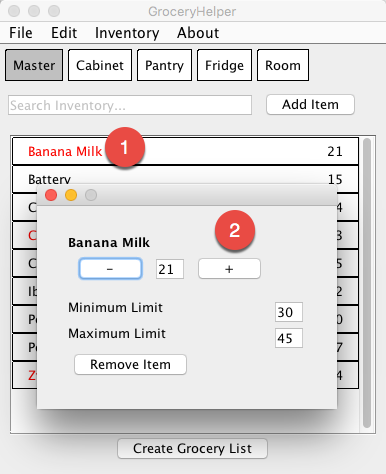
\includegraphics[scale=0.4]{20.png}}

Any of the fields can be changed by entering a new number that meets the requirements above. If the minimum limit is changed to a number greater than the maximum limit or vice versa, a window will pop up explaining that one of these values must be changed. Additionally, the quantity can be changed with the \menu{+} and \menu{-} buttons on either side of the text field. Each click of these buttons increment and decrement the quantity of the item by 1, respectively.
		
		\subsubsection{Removing Items}
To remove an item, click on its name in the display. At the bottom of the frame that pops up, click on the \menu{Remove Item} button. A window will verify whether the user is sure he/she wants to remove the item. If the \menu{Yes} button is clicked, the item will be removed from the inventory.\\

\centerline{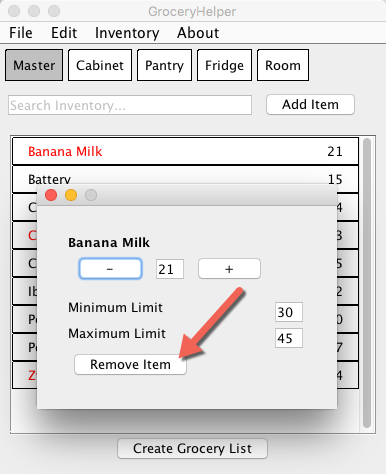
\includegraphics[scale=0.5]{13.png}}


	\subsection{Grocery List}
		The central feature of GroceryHelper is the Grocery List function. The grocery list is exactly what it sounds like: a list that is conveniently generated by the program which outlines the quantity of each item that the user must purchase to reach every item's maximum limit.

Sometimes, a user might wish to only replenish a certain inventory. For such a case, a grocery list can be easily generated for each specific inventory, as well as all of the inventories (the Master inventory). This can be achieved by simply navigating to the desired inventory and pressing the \menu{Create Grocery List} button on the bottom of the window. \\

\centerline{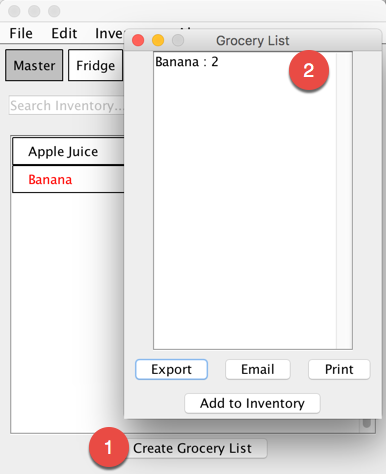
\includegraphics[scale=0.5]{09.png}}


Once the groceries on the list have been purchased, use the \menu{Add to Inventory} to change the quantities of all items on the list to their new values.

		\subsubsection{Export List to a File}
	A grocery list can also be saved to a file. There are two ways to save a grocery list:
		
\begin{enumerate}
\item In the top menu, navigate to \menu[,]{File, Export Grocery List, File}.
\item Press the \menu{Export} button at the bottom of the grocery list window.

\end{enumerate}		

\centerline{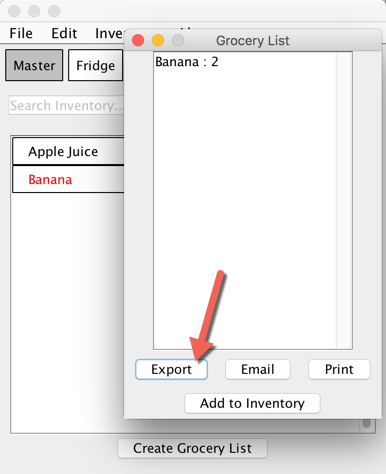
\includegraphics[scale=0.5]{21.png}}

\pagebreak

		
		In any case, select a location to save the file, enter a name for it, and choose a format, a Microsoft Word Document (.docx) or a Plain Text File (.txt), and click \menu{Save}.\\
		
	\centerline{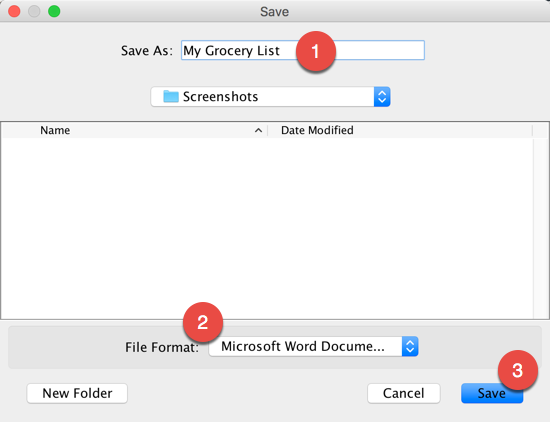
\includegraphics[scale=0.5]{15.png}}

		
		 
		
		\subsubsection{Printing}
Grocery lists can also be printed without being saved to a file. This feature is useful when a user prefers to have a hard copy of the grocery list when going shopping. There are three ways to print grocery lists:

\begin{enumerate}
\item In the menu bar, navigate to \menu[,]{File, Print}. 
\item From the grocery list window, click the \menu{Print} button. A window will pop up prompting the user to select a printer.
\item Use the keyboard shortcut \keys{\ctrlwin + P} on Windows or \keys{\cmd + P} on Mac.
\end{enumerate}
		
		
	\centerline{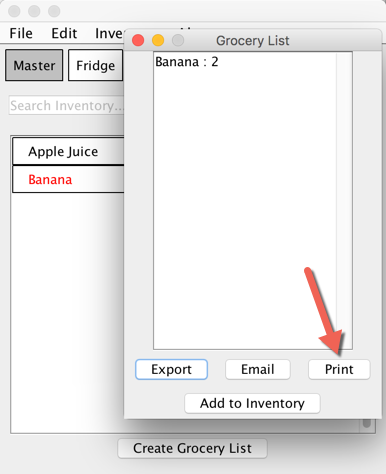
\includegraphics[scale=0.5]{03.png}}
	
	
	The following is an example of a printed grocery list. \\
	
	\centerline{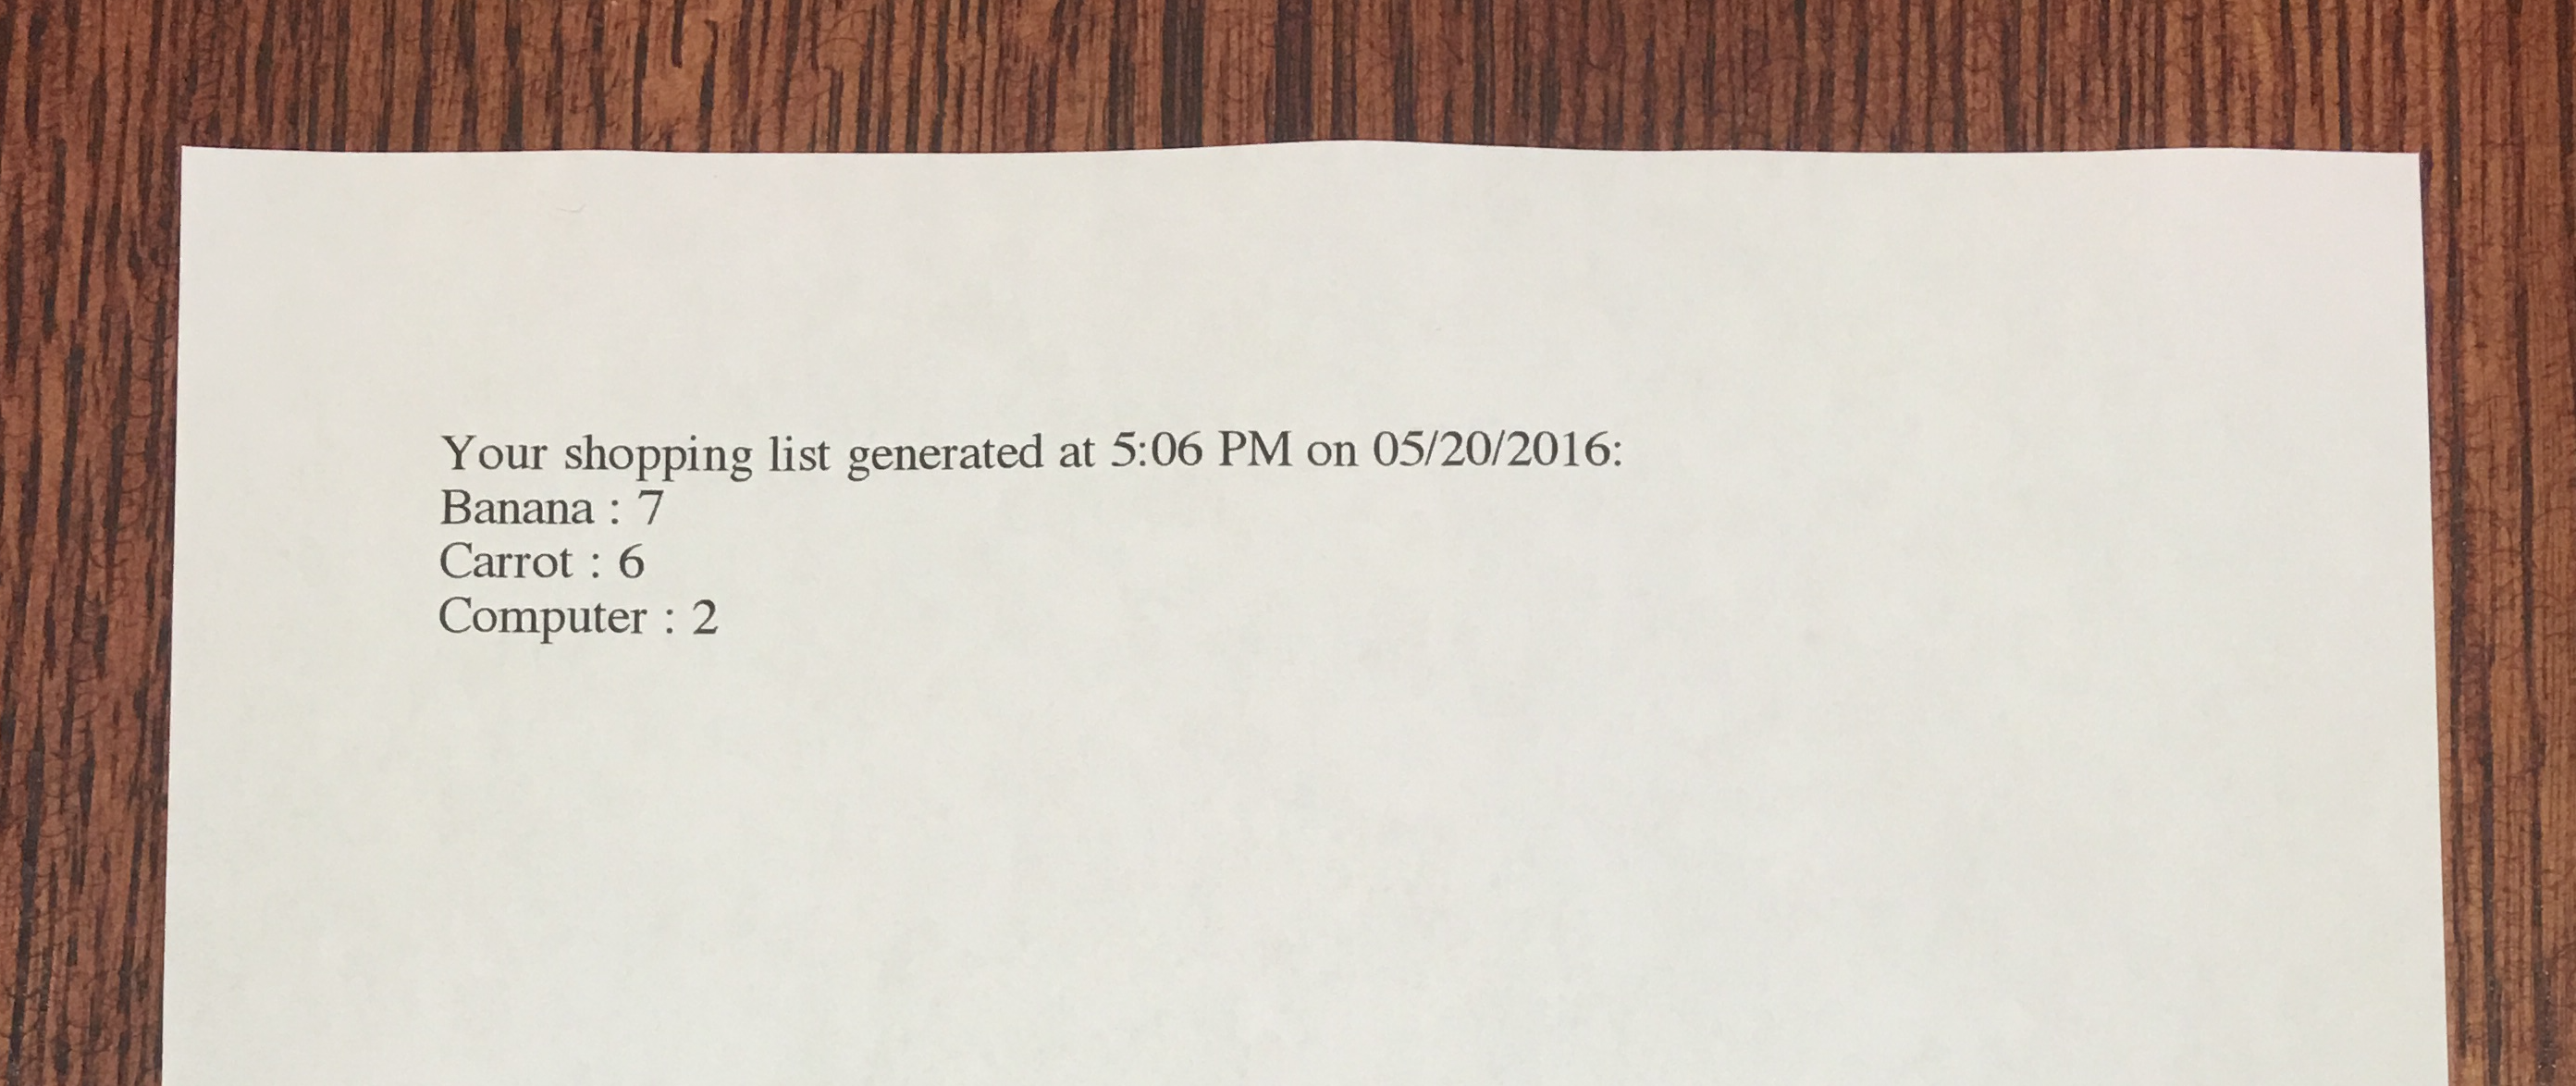
\includegraphics[width=0.5\textwidth]{crop.png}}
		
		
		\subsubsection{Emailing}
Grocery lists can also be emailed to any valid email address. This feature is useful when a user prefers to have an electronic version of the grocery list to refer to while shopping. The grocery list can also be sent to a friend or family member to remind him/her of products to purchase, just in case he/she to bring or misplaced his/her grocery list. 

There are two ways to email grocery lists:

\begin{enumerate}
\item Navigate to \menu[,]{File, Export Grocery List, Email}. 
\item Press \menu{Create Grocery List}. Confirm the generated grocery list, then press the \menu{Email} button at the bottom of the grocery list window.
\end{enumerate}

In any case, a window will pop up prompting the user for an email address. An email containing the grocery list will be sent to the email address entered in the window. The email will be from \verb|mxshoppinglist@gmail.com|; please add this email address to your contacts in order to prevent your grocery lists from being interpreted as spam.\\

	\centerline{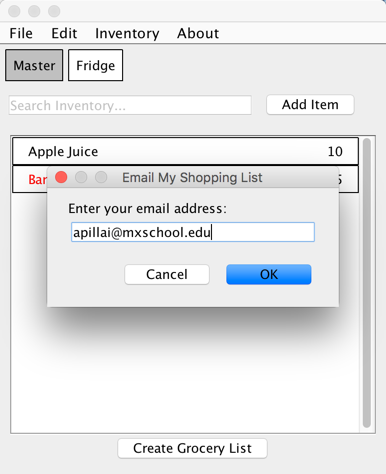
\includegraphics[scale=0.5]{19.png}}

	\centerline{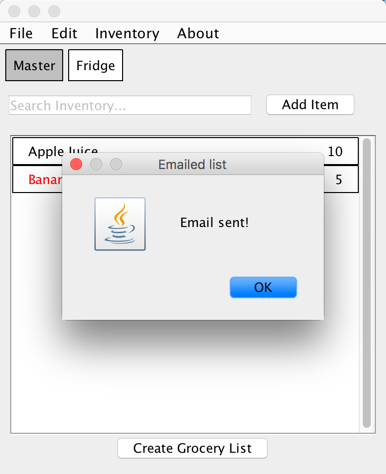
\includegraphics[scale=0.5]{16.png}}


If the email address is invalid, GroceryHelper will display a message explaining that a valid email address must be entered.





	\subsection{Undo and Redo Functions}
	
	Mistakes happen, and we at the Wacky Wozniaks Company understand your struggle. Thus, we have taken extra measures to make sure any action a user performs in GroceryHelper can be undone and redone, not unlike most commercial products such as word processors and photo editing software. 
	
	There are two ways to undo an operation:

\begin{enumerate}
\item Navigate to \menu[,]{Edit, Undo}.
\item Use the keyboard shortcut \keys{\ctrlwin + Z} on Windows or \keys{\cmd + Z} on Mac.\\
\end{enumerate}	
	
\centerline{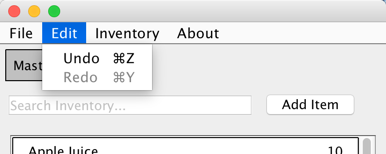
\includegraphics[scale=0.5]{07.png}}	
	
	After undoing an operation, it can also be redone if the user determines that the previously undone operation was the correct decision.
	
\begin{enumerate}
\item Navigate to \menu[,]{Edit, Redo}.
\item Use the keyboard shortcut \keys{\ctrlwin + Y} on Windows or \keys{\cmd + Y} on Mac.
\end{enumerate}	
	
Please be aware that once you undo an operation and perform another operation, previously undone operations are lost, and thus the user cannot perform the redo function.

\pagebreak

\section{Uninstalling GroceryHelper}

Here at the Wacky Wozniaks Company, we take pride in our products, and we truly do hope GroceryHelper has been a useful program to you. However, if you really do wish to uninstall the program, please follow these directions:

\subsection{Windows Users}

\begin{enumerate}
\item Locate \verb|GroceryHelper.exe| (the file used to run the program) and delete it.
\item Open a Search window on your computer. This functionality is likely in your start menu (Windows 7 or below) or your start screen (Windows 8 or newer).
\item Search for the folder \verb|WackyWozniaks|. 
\item Once you locate the folder, usually in your home directory,* delete the folder.   
\end{enumerate}

*Your home directory is most likely located in \verb|C:\Users\[Your Username]|. 

\subsection{Mac OS X Users}
\begin{enumerate}
\item Delete the \verb|GroceryHelper.app| file.
\item Open a new Finder window, then from the menu bar, press ``Go'' then ``Go to Folder''.
\item Type in \verb|~/Library| (without the quotation marks) and press ``Go''.
\item Locate the \verb|WackyWozniaks| folder and delete it.
\end{enumerate}

\subsection{Linux Users}
\begin{enumerate}
\item Run the following command in your terminal: 

\verb|find . -name "WackyWozniaks" -exec rm -r "{}" \;|
\end{enumerate}

Please be aware that misusing the command above may result in a complete wipe of your hard drive. Proceed at your own risk. Alternatively, you can search your home directory manually to see if the \verb|WackyWozniaks| folder is present. If it is, delete that folder, as well as the \verb|.jar| file used to launch the program. 

\pagebreak

\vspace{-0.2in}

\section{Frequently Asked Questions}

\vspace{-0.15in}

After thorough market research, we enlisted various beta testers for whom GroceryHelper may prove useful for managing their household consumable items. In the interest of full disclosure, these adults consist of, but may not be limited to, Ms. E. M. Martineau, Ms. J. A. Mullan, and Dr. E. Woo. The following are some frequently asked questions from this group.


\begin{itemize}
\item[Q.] \textit{\textbf{What are minimum and maximum limits?}}\\

\item[A.] The minimum limit of an item is the lowest value the quantity can be before GroceryHelper will consider you to be ``out of'' that item and add it the grocery list. When an item is placed on a grocery list, the amount GroceryHelper suggests for you to purchase is the amount required to reach the maximum limit.\\

\item[Q.] \textit{\textbf{How can I change the minimum and maximum limits of an item?}}\\

	\item[A.] To change the limits of an item, click on the item's icon. Information about the item will pop up in a new window. Click on the number next to minimum Limit or maximum Limit, delete it, and type in a new one.\\

\item[Q.] \textit{\textbf{Why can I only set quantities to integers? Why can't I use fractions?}}\\

	\item[A.] The current implementation of GroceryHelper only accepts integer quantities to simplify the process of creating grocery lists and updating quantities. A possible solution to your problem would be to change the units you use to represent the quantity, such as representing bread in slices rather than loaves. \\

\item[Q.] \textit{\textbf{How can I move an item to a different inventory?}}\\

\item[A.] Unfortunately, GroceryHelper does not allow you to move an item to another inventory. However, there are only four attributes related to an item, so deleting the item from its current inventory and adding that same item to a different inventory is an easy task.\\

\item [Q.] \textit{\textbf{What do I do if my computer says that my version of Java is outdated or incompatible with GroceryHelper?}}\\

\item[A.] Please go to \verb|https://www.java.com/en| \verb|/download/| and install the latest version of Java. If your computer still says that your version of Java is outdated, unfortunately, your computer may be too outdated to support GroceryHelper. \\

\item [Q.] \textit{\textbf{GroceryHelper won't launch! When I double click the icon, a window flashes for a moment, then goes away.}}\\

\item[A.] In this case, it is highly likely your GroceryHelper data files have been corrupted. Please follow the instructions in this manual on uninstalling GroceryHelper, then download the program again. Please note that this will erase all of your current inventory data.

\end{itemize}

%\pagebreak

\section{Additional Screenshots of GroceryHelper}

This manual utilized screenshots of GroceryHelper taken on a Macintosh computer running Mac OS 10.11.4. However, GroceryHelper can be run on a multitude of platforms, thanks to the innately cross-platform friendly nature of the Java platform. For the sake of demonstration of the program's wide compatibility, the following are a few screenshots of GroceryHelper being utilized on a laptop running Windows Vista Service Pack 1.

\begin{table}[H]
\centering
\begin{tabular}{c c}
\begin{minipage}{0.35\textwidth}
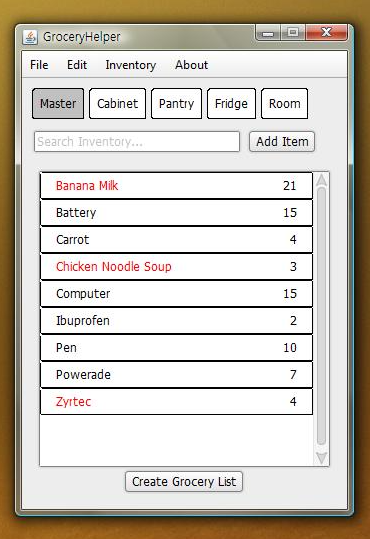
\includegraphics[width=\textwidth]{w01.png}
\end{minipage}

&

\begin{minipage}{0.35\textwidth}
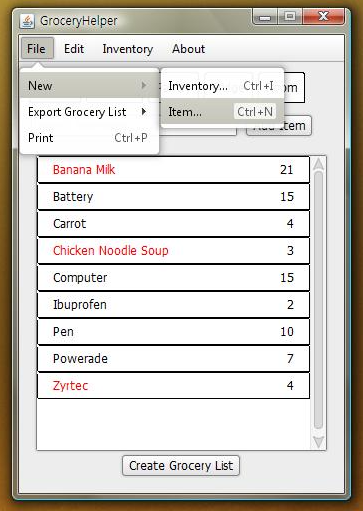
\includegraphics[width=\textwidth]{w03.png}
\end{minipage}

\end{tabular}
\end{table}



\centerline{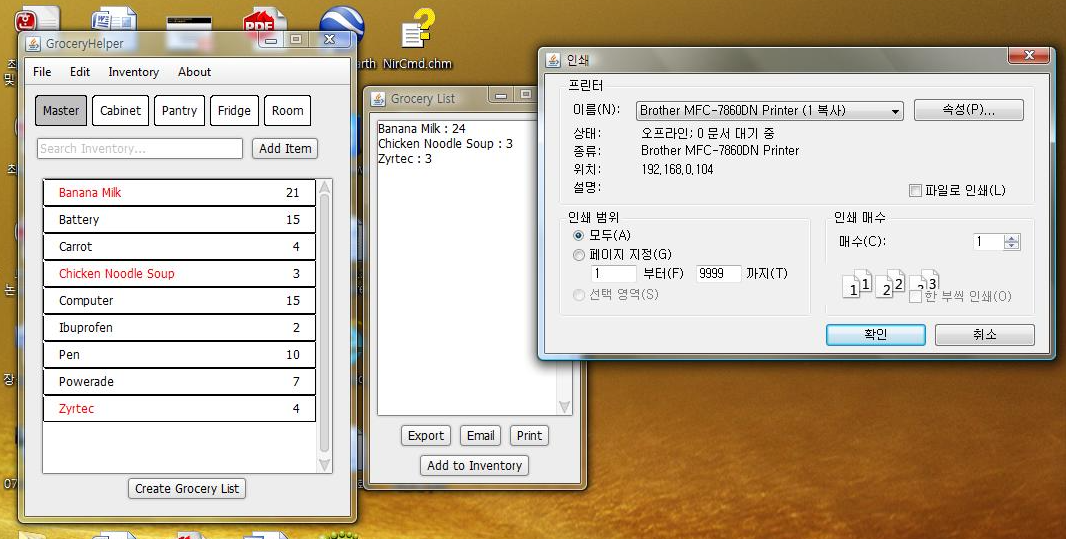
\includegraphics[scale=0.45]{w004.png}}	



\pagebreak

\section{Legal Information}

GroceryHelper{\footnotesize \textsuperscript{TM}} is a trademark of the Wacky Wozniaks Company.

The Wacky Wozniaks Company welcomes users from around the world. If you or someone you know would benefit from a translation of this manual and/or GroceryHelper into a different language, please contact us. We may be able to arrange a special translation for our international customers. 

The attached Software License Agreement is also available in multiple languages. We welcome international use of our products and creation of derivative works, so please do not hesitate to contact us if you might benefit from a copy of the License in a language other than English. 


Oracle and Java are registered trademarks of Oracle and/or its affiliates. Other names may be trademarks of their respective owners.

Intel and Pentium are trademarks or registered trademarks of Intel Corporation.

Microsoft, Microsoft Word, Windows, Windows 10, Windows 8, Windows 7, Windows Vista, Windows XP, Windows Server 2008, and Windows Server 2012 are either registered trademarks or trademarks of Microsoft Corporation in the United States and/or other countries. The formal name of Windows Vista is Microsoft Windows Vista operating system.

Mac, Mac OS, and OS X are trademarks of Apple Inc., registered in the United States and other countries. 

Linux$^\text{\textregistered}$~is the registered trademark of Linus Torvalds in the U.S. and other countries.

GroceryHelper{\footnotesize\textsuperscript{TM}} logo graphics consist of vector graphics by Alfredo Hernandez, Freepik, Baianat, and Madebyoliver from \url{www.flaticon.com}. All copyrighted vector graphics are used lawfully under the Flaticon Basic License, the contents of which can be found on \verb|http://file005.flaticon.com/| \verb|downloads/license/license.pdf|




\pagebreak

\section{Software License Agreement}

\vspace*{-1em}

{\large \textbf{READ CAREFULLY BEFORE USING!}}

{\fontsize{6}{6}\selectfont

IMPORTANT - READ THIS AGREEMENT BEFORE USING GROCERYHELPER (THE ``SOFTWARE''). BY USING THE SOFTWARE, YOU AGREE TO BE BOUND BY TERMS OF THIS AGREEMENT.
ENGLISH 

\textcopyright 2016, The Wacky Wozniaks Company, All Rights Reserved

GroceryHelper{\fontsize{5.5}{5.5}\selectfont \textsuperscript{TM}} is a trademark of the Wacky Wozniaks Company.

\begin{center}
End User Software License Agreement For GroceryHelper


GNU GENERAL PUBLIC LICENSE

Version 3, 29 June 2007
\end{center}

Copyright \textcopyright 2007 Free Software Foundation, Inc. $<$http://fsf.org/$>$

Everyone is permitted to copy and distribute verbatim copies of this license document, but changing it is not allowed.

\textbf{Preamble}

The GNU General Public License is a free, copyleft license for software and other kinds of works.

The licenses for most software and other practical works are designed to take away your freedom to share and change the works. By contrast, the GNU General Public License is intended to guarantee your freedom to share and change all versions of a program--to make sure it remains free software for all its users. We, the Free Software Foundation, use the GNU General Public License for most of our software; it applies also to any other work released this way by its authors. You can apply it to your programs, too.

When we speak of free software, we are referring to freedom, not price. Our General Public Licenses are designed to make sure that you have the freedom to distribute copies of free software (and charge for them if you wish), that you receive source code or can get it if you want it, that you can change the software or use pieces of it in new free programs, and that you know you can do these things.

To protect your rights, we need to prevent others from denying you these rights or asking you to surrender the rights. Therefore, you have certain responsibilities if you distribute copies of the software, or if you modify it: responsibilities to respect the freedom of others.

For example, if you distribute copies of such a program, whether gratis or for a fee, you must pass on to the recipients the same freedoms that you received. You must make sure that they, too, receive or can get the source code. And you must show them these terms so they know their rights.

Developers that use the GNU GPL protect your rights with two steps: (1) assert copyright on the software, and (2) offer you this License giving you legal permission to copy, distribute and/or modify it.

For the developers' and authors' protection, the GPL clearly explains that there is no warranty for this free software. For both users' and authors' sake, the GPL requires that modified versions be marked as changed, so that their problems will not be attributed erroneously to authors of previous versions.

Some devices are designed to deny users access to install or run modified versions of the software inside them, although the manufacturer can do so. This is fundamentally incompatible with the aim of protecting users' freedom to change the software. The systematic pattern of such abuse occurs in the area of products for individuals to use, which is precisely where it is most unacceptable. Therefore, we have designed this version of the GPL to prohibit the practice for those products. If such problems arise substantially in other domains, we stand ready to extend this provision to those domains in future versions of the GPL, as needed to protect the freedom of users.

Finally, every program is threatened constantly by software patents. States should not allow patents to restrict development and use of software on general-purpose computers, but in those that do, we wish to avoid the special danger that patents applied to a free program could make it effectively proprietary. To prevent this, the GPL assures that patents cannot be used to render the program non-free.

The precise terms and conditions for copying, distribution and modification follow.

\textbf{TERMS AND CONDITIONS}

0. Definitions.

``This License'' refers to version 3 of the GNU General Public License.

``Copyright'' also means copyright-like laws that apply to other kinds of works, such as semiconductor masks.

``The Program'' refers to any copyrightable work licensed under this License. Each licensee is addressed as ``you''. ``Licensees'' and ``recipients'' may be individuals or organizations.

To ``modify'' a work means to copy from or adapt all or part of the work in a fashion requiring copyright permission, other than the making of an exact copy. The resulting work is called a ``modified version'' of the earlier work or a work ``based on'' the earlier work.

A ``covered work'' means either the unmodified Program or a work based on the Program.

To ``propagate'' a work means to do anything with it that, without permission, would make you directly or secondarily liable for infringement under applicable copyright law, except executing it on a computer or modifying a private copy. Propagation includes copying, distribution (with or without modification), making available to the public, and in some countries other activities as well.

To ``convey'' a work means any kind of propagation that enables other parties to make or receive copies. Mere interaction with a user through a computer network, with no transfer of a copy, is not conveying.

An interactive user interface displays ``Appropriate Legal Notices'' to the extent that it includes a convenient and prominently visible feature that (1) displays an appropriate copyright notice, and (2) tells the user that there is no warranty for the work (except to the extent that warranties are provided), that licensees may convey the work under this License, and how to view a copy of this License. If the interface presents a list of user commands or options, such as a menu, a prominent item in the list meets this criterion.

1. Source Code.

The ``source code'' for a work means the preferred form of the work for making modifications to it. ``Object code'' means any non-source form of a work.

A ``Standard Interface'' means an interface that either is an official standard defined by a recognized standards body, or, in the case of interfaces specified for a particular programming language, one that is widely used among developers working in that language.

The ``System Libraries'' of an executable work include anything, other than the work as a whole, that (a) is included in the normal form of packaging a Major Component, but which is not part of that Major Component, and (b) serves only to enable use of the work with that Major Component, or to implement a Standard Interface for which an implementation is available to the public in source code form. A ``Major Component'', in this context, means a major essential component (kernel, window system, and so on) of the specific operating system (if any) on which the executable work runs, or a compiler used to produce the work, or an object code interpreter used to run it.

The ``Corresponding Source'' for a work in object code form means all the source code needed to generate, install, and (for an executable work) run the object code and to modify the work, including scripts to control those activities. However, it does not include the work's System Libraries, or general-purpose tools or generally available free programs which are used unmodified in performing those activities but which are not part of the work. For example, Corresponding Source includes interface definition files associated with source files for the work, and the source code for shared libraries and dynamically linked subprograms that the work is specifically designed to require, such as by intimate data communication or control flow between those subprograms and other parts of the work.

The Corresponding Source need not include anything that users can regenerate automatically from other parts of the Corresponding Source.

The Corresponding Source for a work in source code form is that same work.

2. Basic Permissions.

All rights granted under this License are granted for the term of copyright on the Program, and are irrevocable provided the stated conditions are met. This License explicitly affirms your unlimited permission to run the unmodified Program. The output from running a covered work is covered by this License only if the output, given its content, constitutes a covered work. This License acknowledges your rights of fair use or other equivalent, as provided by copyright law.

You may make, run and propagate covered works that you do not convey, without conditions so long as your license otherwise remains in force. You may convey covered works to others for the sole purpose of having them make modifications exclusively for you, or provide you with facilities for running those works, provided that you comply with the terms of this License in conveying all material for which you do not control copyright. Those thus making or running the covered works for you must do so exclusively on your behalf, under your direction and control, on terms that prohibit them from making any copies of your copyrighted material outside their relationship with you.

Conveying under any other circumstances is permitted solely under the conditions stated below. Sublicensing is not allowed; section 10 makes it unnecessary.

3. Protecting Users' Legal Rights From Anti-Circumvention Law.

No covered work shall be deemed part of an effective technological measure under any applicable law fulfilling obligations under article 11 of the WIPO copyright treaty adopted on 20 December 1996, or similar laws prohibiting or restricting circumvention of such measures.

When you convey a covered work, you waive any legal power to forbid circumvention of technological measures to the extent such circumvention is effected by exercising rights under this License with respect to the covered work, and you disclaim any intention to limit operation or modification of the work as a means of enforcing, against the work's users, your or third parties' legal rights to forbid circumvention of technological measures.

4. Conveying Verbatim Copies.

You may convey verbatim copies of the Program's source code as you receive it, in any medium, provided that you conspicuously and appropriately publish on each copy an appropriate copyright notice; keep intact all notices stating that this License and any non-permissive terms added in accord with section 7 apply to the code; keep intact all notices of the absence of any warranty; and give all recipients a copy of this License along with the Program.

You may charge any price or no price for each copy that you convey, and you may offer support or warranty protection for a fee.

5. Conveying Modified Source Versions.

You may convey a work based on the Program, or the modifications to produce it from the Program, in the form of source code under the terms of section 4, provided that you also meet all of these conditions:

a) The work must carry prominent notices stating that you modified it, and giving a relevant date.
b) The work must carry prominent notices stating that it is released under this License and any conditions added under section 7. This requirement modifies the requirement in section 4 to ``keep intact all notices''.
c) You must license the entire work, as a whole, under this License to anyone who comes into possession of a copy. This License will therefore apply, along with any applicable section 7 additional terms, to the whole of the work, and all its parts, regardless of how they are packaged. This License gives no permission to license the work in any other way, but it does not invalidate such permission if you have separately received it.
d) If the work has interactive user interfaces, each must display Appropriate Legal Notices; however, if the Program has interactive interfaces that do not display Appropriate Legal Notices, your work need not make them do so.
A compilation of a covered work with other separate and independent works, which are not by their nature extensions of the covered work, and which are not combined with it such as to form a larger program, in or on a volume of a storage or distribution medium, is called an ``aggregate'' if the compilation and its resulting copyright are not used to limit the access or legal rights of the compilation's users beyond what the individual works permit. Inclusion of a covered work in an aggregate does not cause this License to apply to the other parts of the aggregate.

6. Conveying Non-Source Forms.

You may convey a covered work in object code form under the terms of sections 4 and 5, provided that you also convey the machine-readable Corresponding Source under the terms of this License, in one of these ways:

a) Convey the object code in, or embodied in, a physical product (including a physical distribution medium), accompanied by the Corresponding Source fixed on a durable physical medium customarily used for software interchange.
b) Convey the object code in, or embodied in, a physical product (including a physical distribution medium), accompanied by a written offer, valid for at least three years and valid for as long as you offer spare parts or customer support for that product model, to give anyone who possesses the object code either (1) a copy of the Corresponding Source for all the software in the product that is covered by this License, on a durable physical medium customarily used for software interchange, for a price no more than your reasonable cost of physically performing this conveying of source, or (2) access to copy the Corresponding Source from a network server at no charge.
c) Convey individual copies of the object code with a copy of the written offer to provide the Corresponding Source. This alternative is allowed only occasionally and noncommercially, and only if you received the object code with such an offer, in accord with subsection 6b.
d) Convey the object code by offering access from a designated place (gratis or for a charge), and offer equivalent access to the Corresponding Source in the same way through the same place at no further charge. You need not require recipients to copy the Corresponding Source along with the object code. If the place to copy the object code is a network server, the Corresponding Source may be on a different server (operated by you or a third party) that supports equivalent copying facilities, provided you maintain clear directions next to the object code saying where to find the Corresponding Source. Regardless of what server hosts the Corresponding Source, you remain obligated to ensure that it is available for as long as needed to satisfy these requirements.
e) Convey the object code using peer-to-peer transmission, provided you inform other peers where the object code and Corresponding Source of the work are being offered to the general public at no charge under subsection 6d.
A separable portion of the object code, whose source code is excluded from the Corresponding Source as a System Library, need not be included in conveying the object code work.

A ``User Product'' is either (1) a ``consumer product'', which means any tangible personal property which is normally used for personal, family, or household purposes, or (2) anything designed or sold for incorporation into a dwelling. In determining whether a product is a consumer product, doubtful cases shall be resolved in favor of coverage. For a particular product received by a particular user, ``normally used'' refers to a typical or common use of that class of product, regardless of the status of the particular user or of the way in which the particular user actually uses, or expects or is expected to use, the product. A product is a consumer product regardless of whether the product has substantial commercial, industrial or non-consumer uses, unless such uses represent the only significant mode of use of the product.

``Installation Information'' for a User Product means any methods, procedures, authorization keys, or other information required to install and execute modified versions of a covered work in that User Product from a modified version of its Corresponding Source. The information must suffice to ensure that the continued functioning of the modified object code is in no case prevented or interfered with solely because modification has been made.

If you convey an object code work under this section in, or with, or specifically for use in, a User Product, and the conveying occurs as part of a transaction in which the right of possession and use of the User Product is transferred to the recipient in perpetuity or for a fixed term (regardless of how the transaction is characterized), the Corresponding Source conveyed under this section must be accompanied by the Installation Information. But this requirement does not apply if neither you nor any third party retains the ability to install modified object code on the User Product (for example, the work has been installed in ROM).

The requirement to provide Installation Information does not include a requirement to continue to provide support service, warranty, or updates for a work that has been modified or installed by the recipient, or for the User Product in which it has been modified or installed. Access to a network may be denied when the modification itself materially and adversely affects the operation of the network or violates the rules and protocols for communication across the network.

Corresponding Source conveyed, and Installation Information provided, in accord with this section must be in a format that is publicly documented (and with an implementation available to the public in source code form), and must require no special password or key for unpacking, reading or copying.

7. Additional Terms.

``Additional permissions'' are terms that supplement the terms of this License by making exceptions from one or more of its conditions. Additional permissions that are applicable to the entire Program shall be treated as though they were included in this License, to the extent that they are valid under applicable law. If additional permissions apply only to part of the Program, that part may be used separately under those permissions, but the entire Program remains governed by this License without regard to the additional permissions.

When you convey a copy of a covered work, you may at your option remove any additional permissions from that copy, or from any part of it. (Additional permissions may be written to require their own removal in certain cases when you modify the work.) You may place additional permissions on material, added by you to a covered work, for which you have or can give appropriate copyright permission.

Notwithstanding any other provision of this License, for material you add to a covered work, you may (if authorized by the copyright holders of that material) supplement the terms of this License with terms:

a) Disclaiming warranty or limiting liability differently from the terms of sections 15 and 16 of this License; or
b) Requiring preservation of specified reasonable legal notices or author attributions in that material or in the Appropriate Legal Notices displayed by works containing it; or
c) Prohibiting misrepresentation of the origin of that material, or requiring that modified versions of such material be marked in reasonable ways as different from the original version; or
d) Limiting the use for publicity purposes of names of licensors or authors of the material; or
e) Declining to grant rights under trademark law for use of some trade names, trademarks, or service marks; or
f) Requiring indemnification of licensors and authors of that material by anyone who conveys the material (or modified versions of it) with contractual assumptions of liability to the recipient, for any liability that these contractual assumptions directly impose on those licensors and authors.
All other non-permissive additional terms are considered ``further restrictions'' within the meaning of section 10. If the Program as you received it, or any part of it, contains a notice stating that it is governed by this License along with a term that is a further restriction, you may remove that term. If a license document contains a further restriction but permits relicensing or conveying under this License, you may add to a covered work material governed by the terms of that license document, provided that the further restriction does not survive such relicensing or conveying.

If you add terms to a covered work in accord with this section, you must place, in the relevant source files, a statement of the additional terms that apply to those files, or a notice indicating where to find the applicable terms.

Additional terms, permissive or non-permissive, may be stated in the form of a separately written license, or stated as exceptions; the above requirements apply either way.

8. Termination.

You may not propagate or modify a covered work except as expressly provided under this License. Any attempt otherwise to propagate or modify it is void, and will automatically terminate your rights under this License (including any patent licenses granted under the third paragraph of section 11).

However, if you cease all violation of this License, then your license from a particular copyright holder is reinstated (a) provisionally, unless and until the copyright holder explicitly and finally terminates your license, and (b) permanently, if the copyright holder fails to notify you of the violation by some reasonable means prior to 60 days after the cessation.

Moreover, your license from a particular copyright holder is reinstated permanently if the copyright holder notifies you of the violation by some reasonable means, this is the first time you have received notice of violation of this License (for any work) from that copyright holder, and you cure the violation prior to 30 days after your receipt of the notice.

Termination of your rights under this section does not terminate the licenses of parties who have received copies or rights from you under this License. If your rights have been terminated and not permanently reinstated, you do not qualify to receive new licenses for the same material under section 10.

9. Acceptance Not Required for Having Copies.

You are not required to accept this License in order to receive or run a copy of the Program. Ancillary propagation of a covered work occurring solely as a consequence of using peer-to-peer transmission to receive a copy likewise does not require acceptance. However, nothing other than this License grants you permission to propagate or modify any covered work. These actions infringe copyright if you do not accept this License. Therefore, by modifying or propagating a covered work, you indicate your acceptance of this License to do so.

10. Automatic Licensing of Downstream Recipients.

Each time you convey a covered work, the recipient automatically receives a license from the original licensors, to run, modify and propagate that work, subject to this License. You are not responsible for enforcing compliance by third parties with this License.

An ``entity transaction'' is a transaction transferring control of an organization, or substantially all assets of one, or subdividing an organization, or merging organizations. If propagation of a covered work results from an entity transaction, each party to that transaction who receives a copy of the work also receives whatever licenses to the work the party's predecessor in interest had or could give under the previous paragraph, plus a right to possession of the Corresponding Source of the work from the predecessor in interest, if the predecessor has it or can get it with reasonable efforts.

You may not impose any further restrictions on the exercise of the rights granted or affirmed under this License. For example, you may not impose a license fee, royalty, or other charge for exercise of rights granted under this License, and you may not initiate litigation (including a cross-claim or counterclaim in a lawsuit) alleging that any patent claim is infringed by making, using, selling, offering for sale, or importing the Program or any portion of it.

11. Patents.

A ``contributor'' is a copyright holder who authorizes use under this License of the Program or a work on which the Program is based. The work thus licensed is called the contributor's ``contributor version''.

A contributor's ``essential patent claims'' are all patent claims owned or controlled by the contributor, whether already acquired or hereafter acquired, that would be infringed by some manner, permitted by this License, of making, using, or selling its contributor version, but do not include claims that would be infringed only as a consequence of further modification of the contributor version. For purposes of this definition, ``control'' includes the right to grant patent sublicenses in a manner consistent with the requirements of this License.

Each contributor grants you a non-exclusive, worldwide, royalty-free patent license under the contributor's essential patent claims, to make, use, sell, offer for sale, import and otherwise run, modify and propagate the contents of its contributor version.

In the following three paragraphs, a ``patent license'' is any express agreement or commitment, however denominated, not to enforce a patent (such as an express permission to practice a patent or covenant not to sue for patent infringement). To ``grant'' such a patent license to a party means to make such an agreement or commitment not to enforce a patent against the party.

If you convey a covered work, knowingly relying on a patent license, and the Corresponding Source of the work is not available for anyone to copy, free of charge and under the terms of this License, through a publicly available network server or other readily accessible means, then you must either (1) cause the Corresponding Source to be so available, or (2) arrange to deprive yourself of the benefit of the patent license for this particular work, or (3) arrange, in a manner consistent with the requirements of this License, to extend the patent license to downstream recipients. ``Knowingly relying'' means you have actual knowledge that, but for the patent license, your conveying the covered work in a country, or your recipient's use of the covered work in a country, would infringe one or more identifiable patents in that country that you have reason to believe are valid.

If, pursuant to or in connection with a single transaction or arrangement, you convey, or propagate by procuring conveyance of, a covered work, and grant a patent license to some of the parties receiving the covered work authorizing them to use, propagate, modify or convey a specific copy of the covered work, then the patent license you grant is automatically extended to all recipients of the covered work and works based on it.

A patent license is ``discriminatory'' if it does not include within the scope of its coverage, prohibits the exercise of, or is conditioned on the non-exercise of one or more of the rights that are specifically granted under this License. You may not convey a covered work if you are a party to an arrangement with a third party that is in the business of distributing software, under which you make payment to the third party based on the extent of your activity of conveying the work, and under which the third party grants, to any of the parties who would receive the covered work from you, a discriminatory patent license (a) in connection with copies of the covered work conveyed by you (or copies made from those copies), or (b) primarily for and in connection with specific products or compilations that contain the covered work, unless you entered into that arrangement, or that patent license was granted, prior to 28 March 2007.

Nothing in this License shall be construed as excluding or limiting any implied license or other defenses to infringement that may otherwise be available to you under applicable patent law.

12. No Surrender of Others' Freedom.

If conditions are imposed on you (whether by court order, agreement or otherwise) that contradict the conditions of this License, they do not excuse you from the conditions of this License. If you cannot convey a covered work so as to satisfy simultaneously your obligations under this License and any other pertinent obligations, then as a consequence you may not convey it at all. For example, if you agree to terms that obligate you to collect a royalty for further conveying from those to whom you convey the Program, the only way you could satisfy both those terms and this License would be to refrain entirely from conveying the Program.

13. Use with the GNU Affero General Public License.

Notwithstanding any other provision of this License, you have permission to link or combine any covered work with a work licensed under version 3 of the GNU Affero General Public License into a single combined work, and to convey the resulting work. The terms of this License will continue to apply to the part which is the covered work, but the special requirements of the GNU Affero General Public License, section 13, concerning interaction through a network will apply to the combination as such.

14. Revised Versions of this License.

The Free Software Foundation may publish revised and/or new versions of the GNU General Public License from time to time. Such new versions will be similar in spirit to the present version, but may differ in detail to address new problems or concerns.

Each version is given a distinguishing version number. If the Program specifies that a certain numbered version of the GNU General Public License ``or any later version'' applies to it, you have the option of following the terms and conditions either of that numbered version or of any later version published by the Free Software Foundation. If the Program does not specify a version number of the GNU General Public License, you may choose any version ever published by the Free Software Foundation.

If the Program specifies that a proxy can decide which future versions of the GNU General Public License can be used, that proxy's public statement of acceptance of a version permanently authorizes you to choose that version for the Program.

Later license versions may give you additional or different permissions. However, no additional obligations are imposed on any author or copyright holder as a result of your choosing to follow a later version.

15. Disclaimer of Warranty.

THERE IS NO WARRANTY FOR THE PROGRAM, TO THE EXTENT PERMITTED BY APPLICABLE LAW. EXCEPT WHEN OTHERWISE STATED IN WRITING THE COPYRIGHT HOLDERS AND/OR OTHER PARTIES PROVIDE THE PROGRAM ``AS IS'' WITHOUT WARRANTY OF ANY KIND, EITHER EXPRESSED OR IMPLIED, INCLUDING, BUT NOT LIMITED TO, THE IMPLIED WARRANTIES OF MERCHANTABILITY AND FITNESS FOR A PARTICULAR PURPOSE. THE ENTIRE RISK AS TO THE QUALITY AND PERFORMANCE OF THE PROGRAM IS WITH YOU. SHOULD THE PROGRAM PROVE DEFECTIVE, YOU ASSUME THE COST OF ALL NECESSARY SERVICING, REPAIR OR CORRECTION.

16. Limitation of Liability.

IN NO EVENT UNLESS REQUIRED BY APPLICABLE LAW OR AGREED TO IN WRITING WILL ANY COPYRIGHT HOLDER, OR ANY OTHER PARTY WHO MODIFIES AND/OR CONVEYS THE PROGRAM AS PERMITTED ABOVE, BE LIABLE TO YOU FOR DAMAGES, INCLUDING ANY GENERAL, SPECIAL, INCIDENTAL OR CONSEQUENTIAL DAMAGES ARISING OUT OF THE USE OR INABILITY TO USE THE PROGRAM (INCLUDING BUT NOT LIMITED TO LOSS OF DATA OR DATA BEING RENDERED INACCURATE OR LOSSES SUSTAINED BY YOU OR THIRD PARTIES OR A FAILURE OF THE PROGRAM TO OPERATE WITH ANY OTHER PROGRAMS), EVEN IF SUCH HOLDER OR OTHER PARTY HAS BEEN ADVISED OF THE POSSIBILITY OF SUCH DAMAGES.

17. Interpretation of Sections 15 and 16.

If the disclaimer of warranty and limitation of liability provided above cannot be given local legal effect according to their terms, reviewing courts shall apply local law that most closely approximates an absolute waiver of all civil liability in connection with the Program, unless a warranty or assumption of liability accompanies a copy of the Program in return for a fee.

END OF TERMS AND CONDITIONS


\hrulefill

In addition to the GNU General Public License Version 3 (GPL) above, the following additional terms (``Additional Terms'') have been added pursuant to provisions of Section 7 of the GPL (``Section 7''). In the case of conflict of provisions between the following and the GPL, Section 7 shall prevail in determining the validity of the Additional Terms. If one portion or section of the Additional Terms is deemed unenforceable or invalid, due to Section 7 or otherwise, the remainder will continue to be valid and enforceable.


Disclaimer of Warranties, in addition to Section 15 of the GPL. 

A. If you are a customer who is a consumer (someone who uses the Software outside of your trade, business or profession), you may have legal rights in your country of residence which would prohibit the following limitations from applying to you, and where prohibited they will not apply to you. To find out more about rights, you should contact a local consumer advice organization. 

B. YOU EXPRESSLY ACKNOWLEDGE AND AGREE THAT, TO THE EXTENT PERMITTED BY APPLICABLE LAW, USE OF THE SOFTWARE AND ANY SERVICES PERFORMED BY OR ACCESSED THROUGH THE SOFTWARE IS AT YOUR SOLE RISK AND THAT THE ENTIRE RISK AS TO SATISFACTORY QUALITY, PERFORMANCE, ACCURACY AND EFFORT IS WITH YOU. 

C. TO THE MAXIMUM EXTENT PERMITTED BY APPLICABLE LAW, THE SOFTWARE AND SERVICES ARE PROVIDED ``AS IS'' AND ``AS AVAILABLE'', WITH ALL FAULTS AND WITHOUT WARRANTY OF ANY KIND, AND THE COMPANY AND THE COMPANY'S LICENSORS (COLLECTIVELY REFERRED TO AS ``THE COMPANY'' FOR THE PURPOSES OF SECTIONS 5 AND 6) HEREBY DISCLAIM ALL WARRANTIES AND CONDITIONS WITH RESPECT TO THE APPLE SOFTWARE AND SERVICES, EITHER EXPRESS, IMPLIED OR STATUTORY, INCLUDING, BUT NOT LIMITED TO, THE IMPLIED WARRANTIES AND/OR CONDITIONS OF MERCHANTABILITY, SATISFACTORY QUALITY, FITNESS FOR A PARTICULAR PURPOSE, ACCURACY, QUIET ENJOYMENT, AND NON-INFRINGEMENT OF THIRD PARTY RIGHTS. 

D. THE COMPANY DOES NOT WARRANT AGAINST INTERFERENCE WITH YOUR ENJOYMENT OF THE SOFTWARE AND SERVICES, THAT THE FUNCTIONS CONTAINED IN, OR SERVICES PERFORMED OR PROVIDED BY, THE SOFTWARE WILL MEET YOUR REQUIREMENTS, THAT THE OPERATION OF THE SOFTWARE OR SERVICES WILL BE UNINTERRUPTED OR ERROR-FREE, THAT ANY SERVICES WILL CONTINUE TO BE MADE AVAILABLE, THAT THE APPLE SOFTWARE OR SERVICES WILL BE COMPATIBLE OR WORK WITH ANY THIRD PARTY SOFTWARE, APPLICATIONS OR THIRD PARTY SERVICES, OR THAT DEFECTS IN THE SOFTWARE OR SERVICES WILL BE CORRECTED. INSTALLATION OF THIS SOFTWARE MAY AFFECT THE USABILITY OF THIRD PARTY SOFTWARE, APPLICATIONS, OR THIRD PARTY SERVICES. 

E. YOU FURTHER ACKNOWLEDGE THAT THE SOFTWARE AND SERVICES ARE NOT INTENDED OR SUITABLE FOR USE IN SITUATIONS OR ENVIRONMENTS WHERE THE FAILURE OR TIME DELAYS OF, OR ERRORS OR INACCURACIES IN, THE CONTENT, DATA OR INFORMATION PROVIDED BY THE APPLE SOFTWARE OR SERVICES COULD LEAD TO DEATH, PERSONAL INJURY, OR SEVERE PHYSICAL OR ENVIRONMENTAL DAMAGE, INCLUDING WITHOUT LIMITATION THE OPERATION OF NUCLEAR FACILITIES, AIRCRAFT NAVIGATION OR COMMUNICATION SYSTEMS, AIR TRAFFIC CONTROL, LIFE SUPPORT OR WEAPONS SYSTEMS. 

F. NO ORAL OR WRITTEN INFORMATION OR ADVICE GIVEN BY THE COMPANY SHALL CREATE A WARRANTY. SHOULD THE SOFTWARE OR SERVICES PROVE DEFECTIVE, YOU ASSUME THE ENTIRE COST OF ALL NECESSARY SERVICING, REPAIR OR CORRECTION. SOME JURISDICTIONS DO NOT ALLOW THE EXCLUSION OF IMPLIED WARRANTIES OR LIMITATIONS ON APPLICABLE STATUTORY RIGHTS OF A CONSUMER, SO THE ABOVE EXCLUSION AND LIMITATIONS MAY NOT APPLY TO YOU. 

Limitation of Liability in addition to Section 16 of the GPL. TO THE EXTENT NOT PROHIBITED BY APPLICABLE LAW, IN NO EVENT SHALL THE COMPANY BE LIABLE FOR PERSONAL INJURY, OR ANY INCIDENTAL, SPECIAL, INDIRECT OR CONSEQUENTIAL DAMAGES WHATSOEVER, INCLUDING, WITHOUT LIMITATION, DAMAGES FOR LOSS OF PROFITS, CORRUPTION OR LOSS OF DATA, FAILURE TO TRANSMIT OR RECEIVE ANY DATA OR INFORMATION, BUSINESS INTERRUPTION OR ANY OTHER COMMERCIAL DAMAGES OR LOSSES, ARISING OUT OF OR RELATED TO YOUR USE OR INABILITY TO USE THE SOFTWARE OR SERVICES OR ANY THIRD PARTY SOFTWARE OR APPLICATIONS IN CONJUNCTION WITH THE SOFTWARE OR SERVICES, HOWEVER CAUSED, REGARDLESS OF THE THEORY OF LIABILITY (CONTRACT, TORT OR OTHERWISE) AND EVEN IF THE COMPANY HAS BEEN ADVISED OF THE POSSIBILITY OF SUCH DAMAGES. SOME JURISDICTIONS DO NOT ALLOW THE EXCLUSION OR LIMITATION OF LIABILITY FOR PERSONAL INJURY, OR OF INCIDENTAL OR CONSEQUENTIAL DAMAGES, SO THIS LIMITATION MAY NOT APPLY TO YOU. In no event shall the Company's total liability to you for all damages (other than as may be required by applicable law in cases involving personal injury) exceed the amount of fifty dollars (\$50.00). The foregoing limitations will apply even if the above stated remedy fails of its essential purpose. 

Limitation of Usage of Names. Neither the name of the copyright holder nor the names of its contributors may be used to endorse or promote products derived from this software without specific prior written permission.

END OF GROCERYHELPER SOFTWARE LICENSE AGREEMENT


\end{document}